\pagestyle{fancy}
\headheight 20pt
\lhead{Ph.D. Thesis --- R. Woods}
\rhead{McMaster - Physics \& Astronomy}
\chead{}
\lfoot{}
\cfoot{\thepage}
\rfoot{}
\renewcommand{\headrulewidth}{0.1pt}
\renewcommand{\footrulewidth}{0.1pt}


\chapter{Code Tests}
\label{chap:codetests}
\thispagestyle{fancy}

In this chapter, I present tests to demonstrate the strengths and limitations of the above algorithm.

\section{Glass}
\label{sec:glass}

A glass of particles is a simple way to demonstrate the most basic functionality of the algorithm. Each particle effectively acts to sample the radiation field at a particular point and has an easily calculated exact solution to compare to.

\subsection{Optically Thin}
\label{sec:thinglass}

{TAKE THIS SECTION OUT? TOO SIMPLE?}

In the optically thin case, we simply want to ensure that we obtain a $1/r^2$ dropoff with flux. There should be no errors present in this test case because in the case of a single source, no averaging is needed and both exact luminosity and position of the source is used for every sink.

\begin{equation}
\label{eq:flux}
F = \frac{L}{4\pi r^2}
\end{equation}

\subsection{Optically Thick}
\label{sec:thickglass}

{TAKE THIS SECTION OUT? TOO SIMPLE?}

Like section \ref{sec:thinglass}, this section aims to demonstrate the base ability of the code. In this case, the glass of particles has a roughly homogeneous density and thus the flux is still easily calculated for comparison.

\begin{itemize}
\item The equation for flux in this case is still fairly simple. If we refer to equation \ref{eq:radabsorption}, we can see the theoretical flux is simply equation \ref{eq:flux} multiplied by the exponential of optical depth. See equation \ref{eq:thickflux}.
\item This assumes a homogeneous density field. The glass does not have an exactly homogeneous field, but has little variance from the average.
\item Figure \ref{fig:thickglasserrors} shows the error distribution of the particles.
\item Note that in the case that the density field is exact, the errors reduce down to machine precision. This emphasizes the importance of accurately modeling the density distribution.
\end{itemize}

\begin{equation}
\label{eq:thickflux}
F = \frac{L}{4\pi r^2} \exp{-\tau}
\end{equation}

\begin{figure}
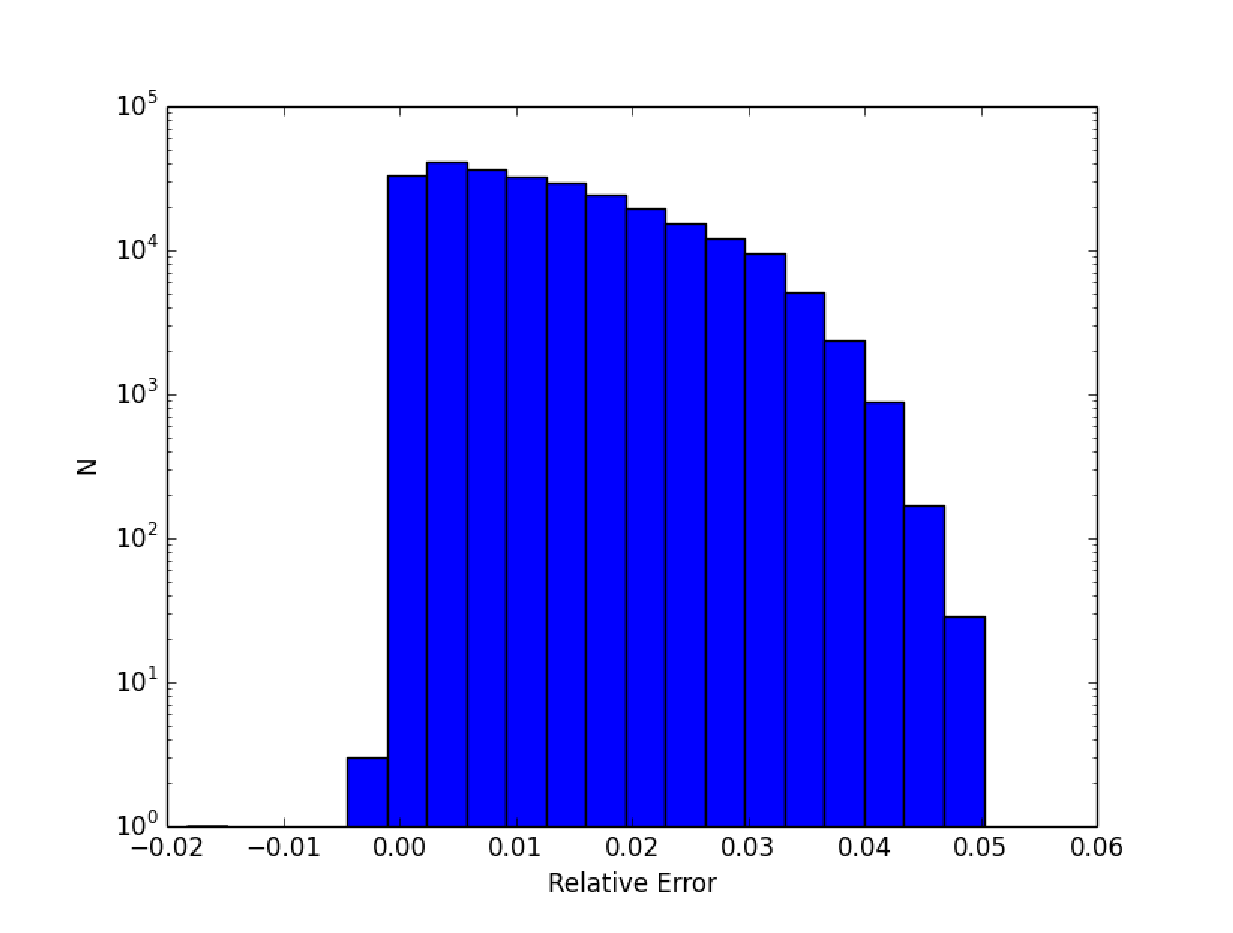
\includegraphics[width=\textwidth]{graphics/error.eps}
\caption[Error distribution for a single source in a uniform field.]{The distribution of flux errors among particles.}
\label{fig:thickglasserrors}
\end{figure}

\section{Multi-Source Glass}
\label{sec:multiglass}

We now show the effect of including many sources. The code is now performing at its most ``stressed;'' having a large number of randomly distributed sources means the code will run at its slowest and will include a large amount of averaging (not quite right).

\begin{itemize}
\item We first present the optically thin case. In this case, the glass has had half of its gas particles replaced with sources so that there are an equal number of each.
\item The error distribution present in this
\end{itemize}

\section{Effects of Averaging the Source}
\label{sec:averagingsource}

We now look closely at what effects averaging sources can have on results.

\subsection{Two star}
\label{sec:twostar}

\begin{figure}
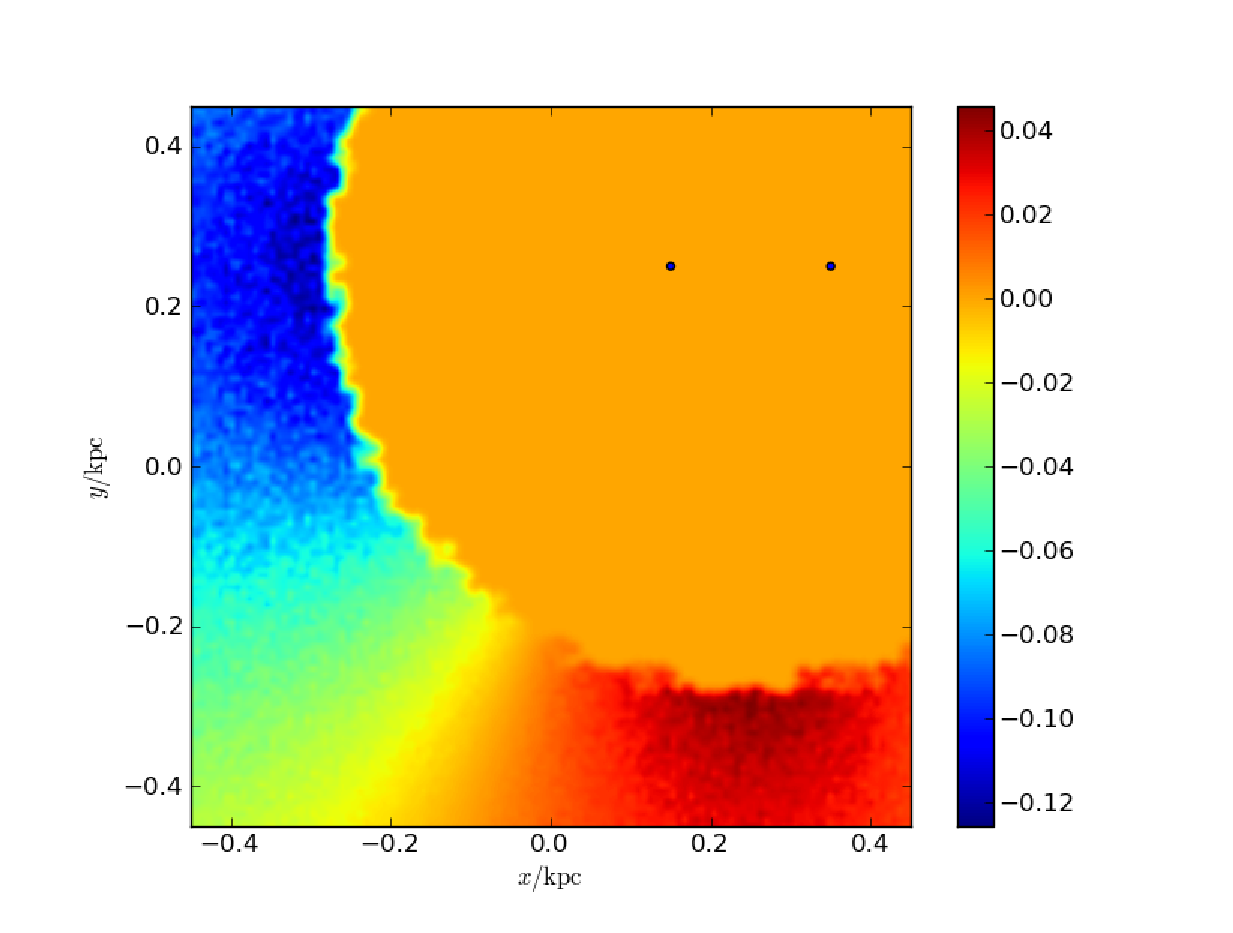
\includegraphics[width=\textwidth]{graphics/errorMap2starthick.eps}
\caption[The error associated with averaging star positions.]{The error associated with averaging star positions.}
\label{fig:twostar}
\end{figure}


\subsection{Isothermal Sphere with a Cluster(?)}
\label{sec:cluster}



\section{The Str\"omgren Sphere}
\label{sec:stromgren}

\begin{equation}
\label{eq:strmogrenradius}
R_S = \left( \frac{3}{4\pi} \frac{\dot{N_{\gamma}}}{\alpha n_H^2}\right)
\end{equation}

\begin{equation}
\label{eq:stromgrentime}
R(t) = R_S[1-\exp{(t/t_{\mbox{recomb}})}]^{1/3}
\end{equation}

\subsection{The Isothermal Case}
\label{sec:isostromgren}

\begin{figure}
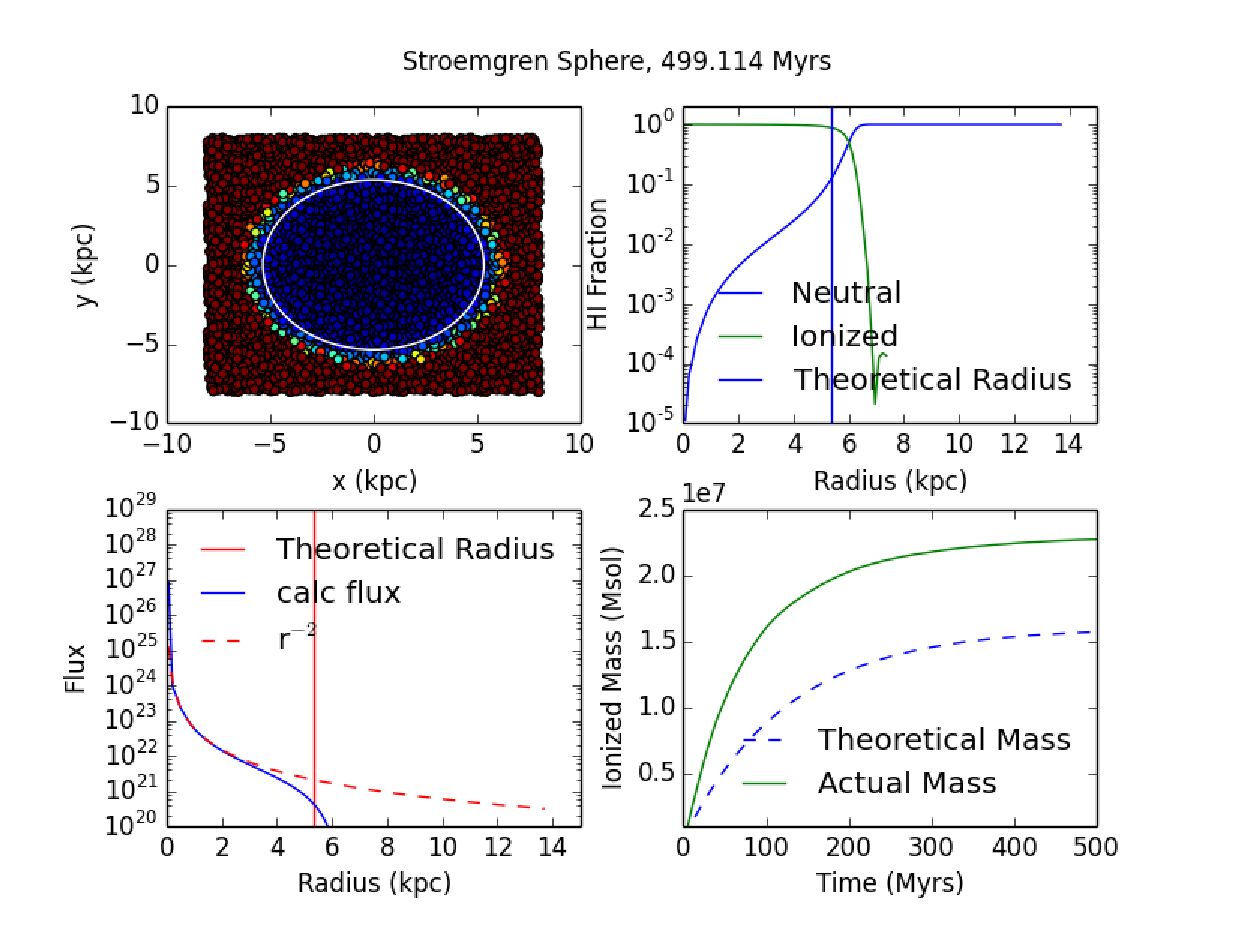
\includegraphics[width=\textwidth]{graphics/ifront6401000.eps}
\caption[The isothermal Str\"omgren Sphere.]{A slice of particles showing the ionization state.}
\label{fig:stromgreniso}
\end{figure}

\subsection{The Thermal Case}
\label{sec:thermalstromgren}

Text to fix the formatting.
\begin{figure}
        \centering
        \begin{subfigure}[b]{0.3\textwidth}
                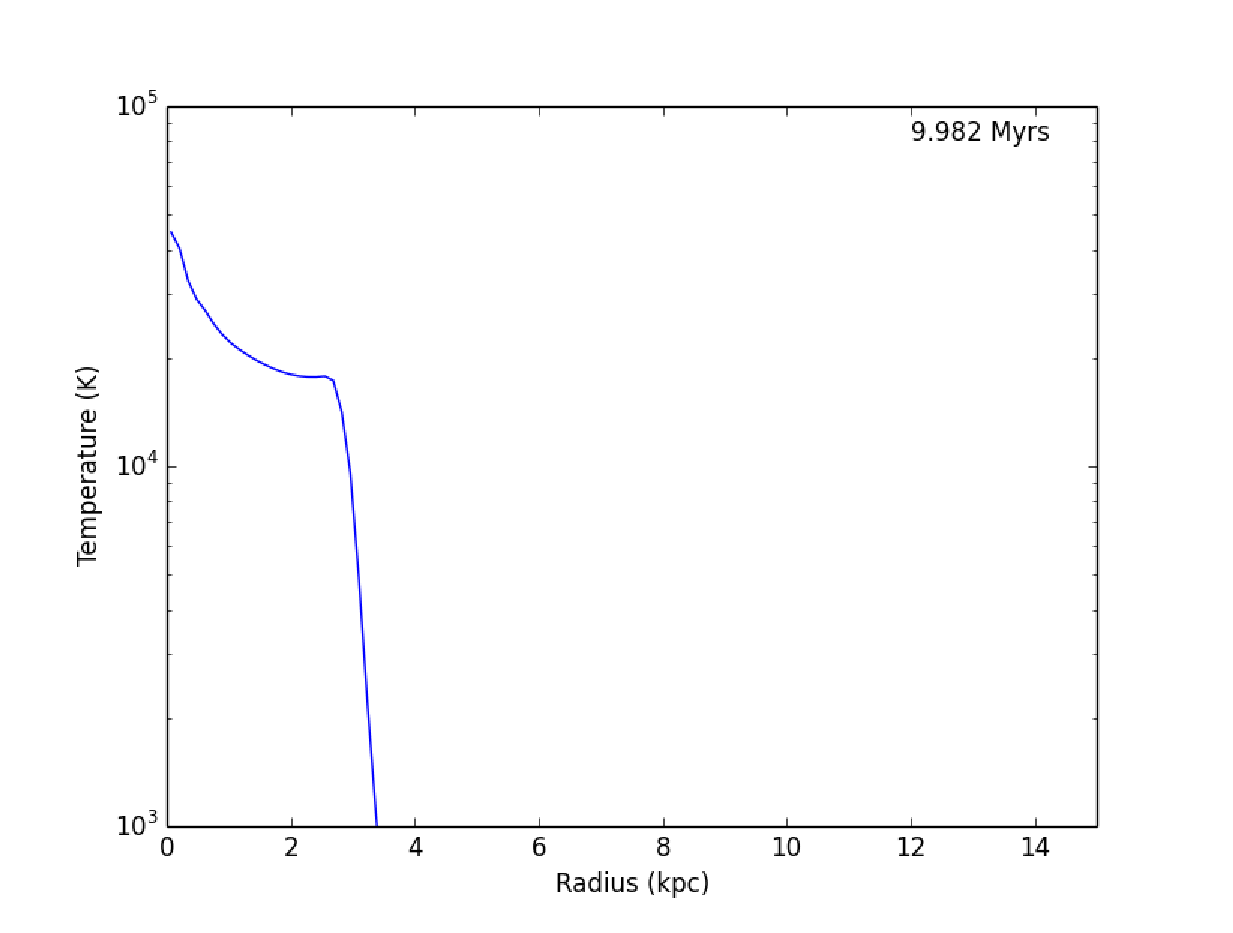
\includegraphics[width=\textwidth]{graphics/ifrontThermal6400020Tempprofile.eps}
                \label{fig:stromgrenthermal10}
        \end{subfigure}
        ~ 
        \begin{subfigure}[b]{0.3\textwidth}
                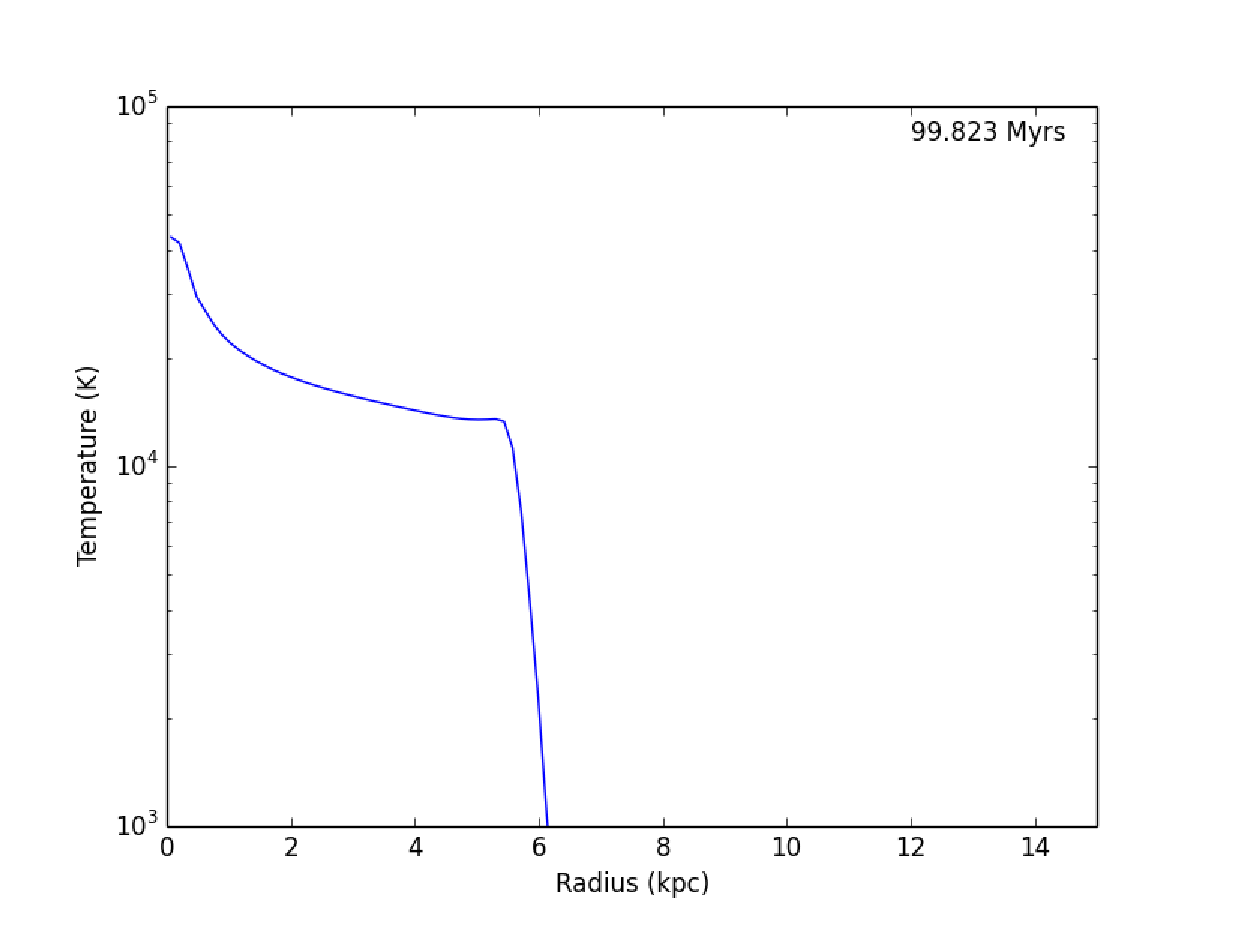
\includegraphics[width=\textwidth]{graphics/ifrontThermal6400200Tempprofile.eps}
                \label{fig:stromgrenthermal100}
        \end{subfigure}
        ~
        \begin{subfigure}[b]{0.3\textwidth}
                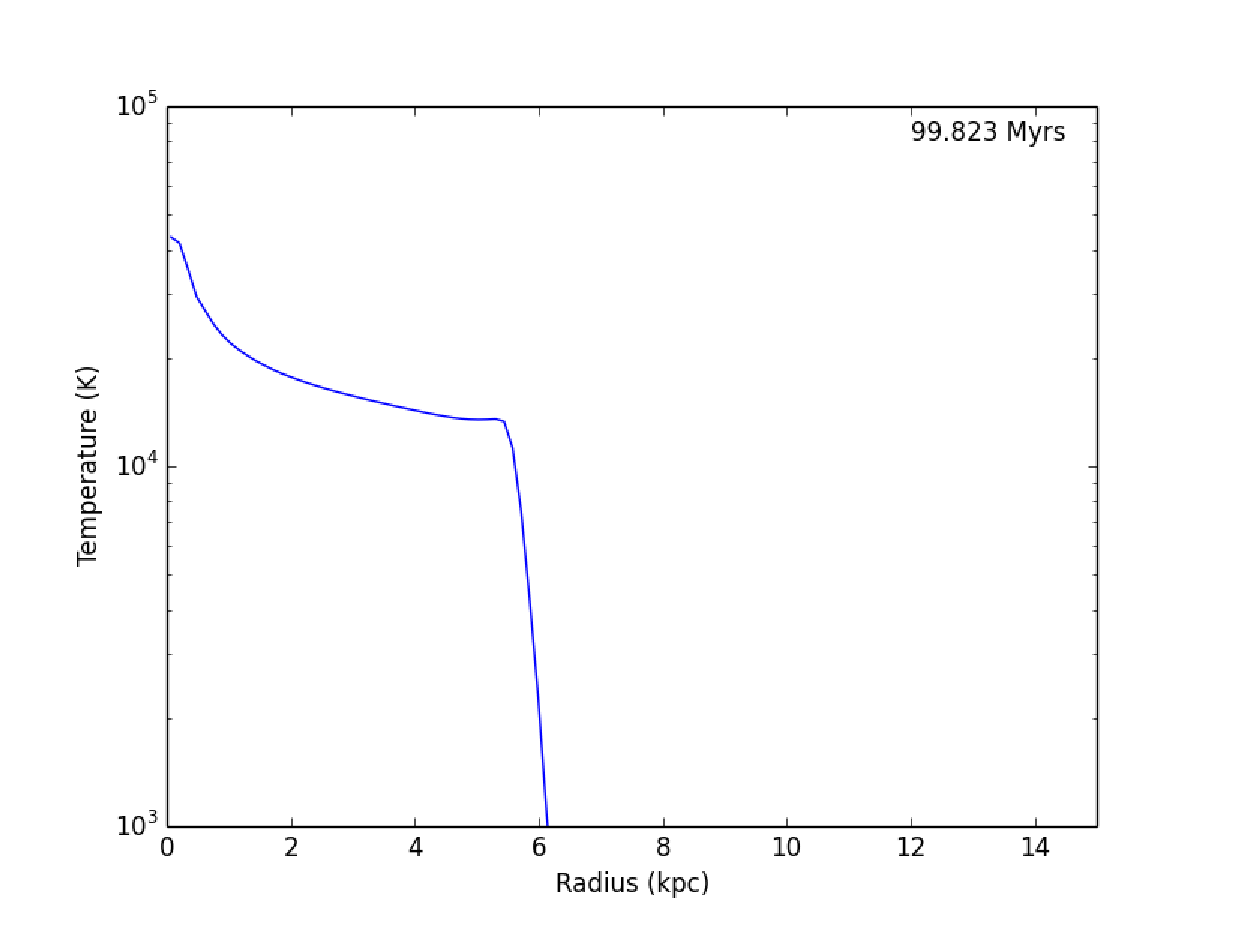
\includegraphics[width=\textwidth]{graphics/ifrontThermal6400200Tempprofile.eps}
                \label{fig:stromgrenthermal500}
        \end{subfigure}
        \caption[Temperature vs radius for the thermal Str\"omgren sphere.]{Temperature vs radius for the thermal Str\"omgren sphere.}
        \label{fig:stromgrenthermal}
\end{figure}

\section{The Gas Wall}
\label{sec:gaswall}

Text to fix the formatting.

\subsection{Only Radiation}
\label{sec:gaswallradonly}

Text to fix the formatting.

\begin{figure}
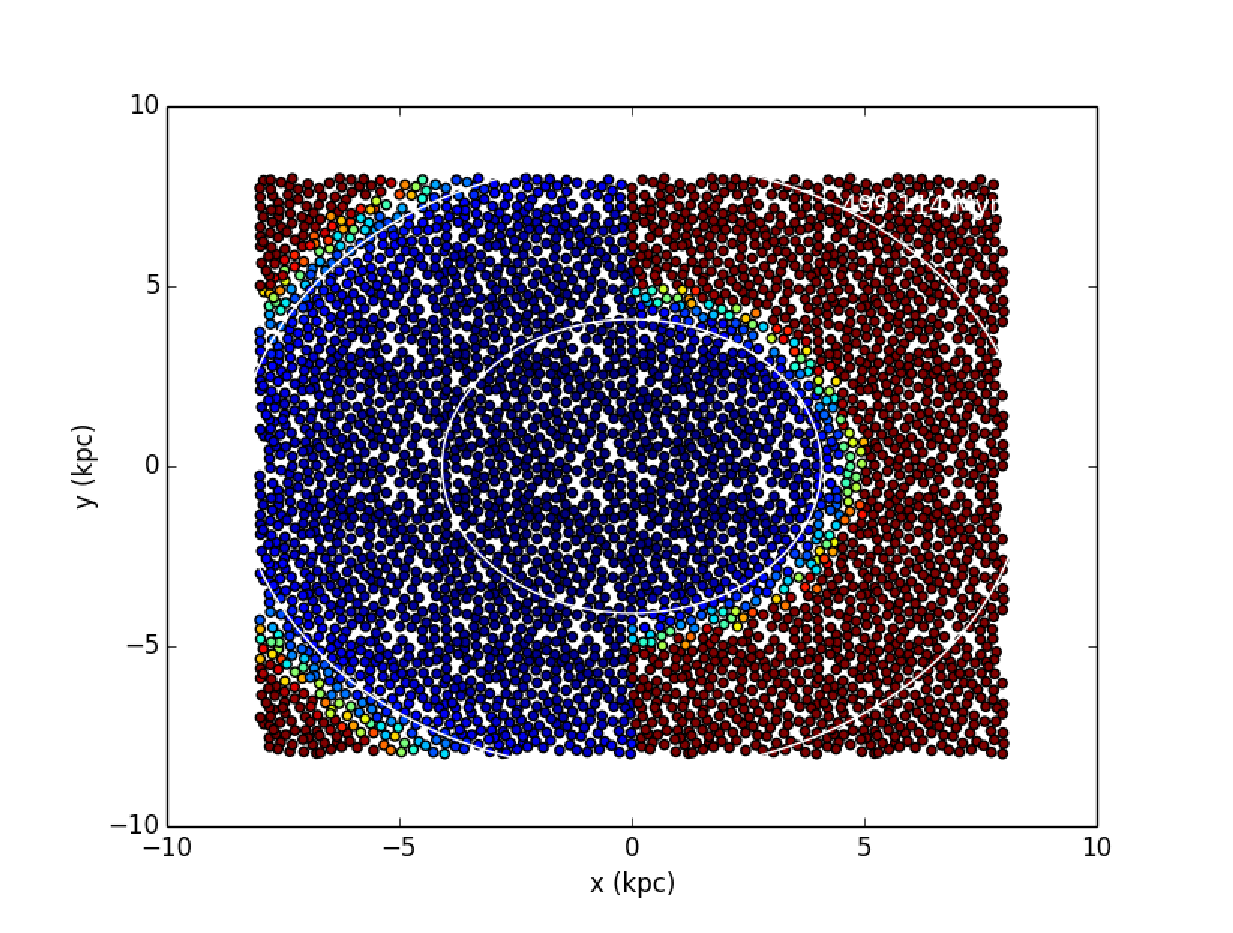
\includegraphics[width=\textwidth]{graphics/gasWall01000HIslice.eps}
\caption[Two slabs of gas at different densities.]{Two slabs of gas at different densities.}
\label{fig:gaswall}
\end{figure}


\subsection{With Hydrodynamics - the Champagne Flow}
\label{sec:champagne}

Text to fix the formatting.

\begin{figure}
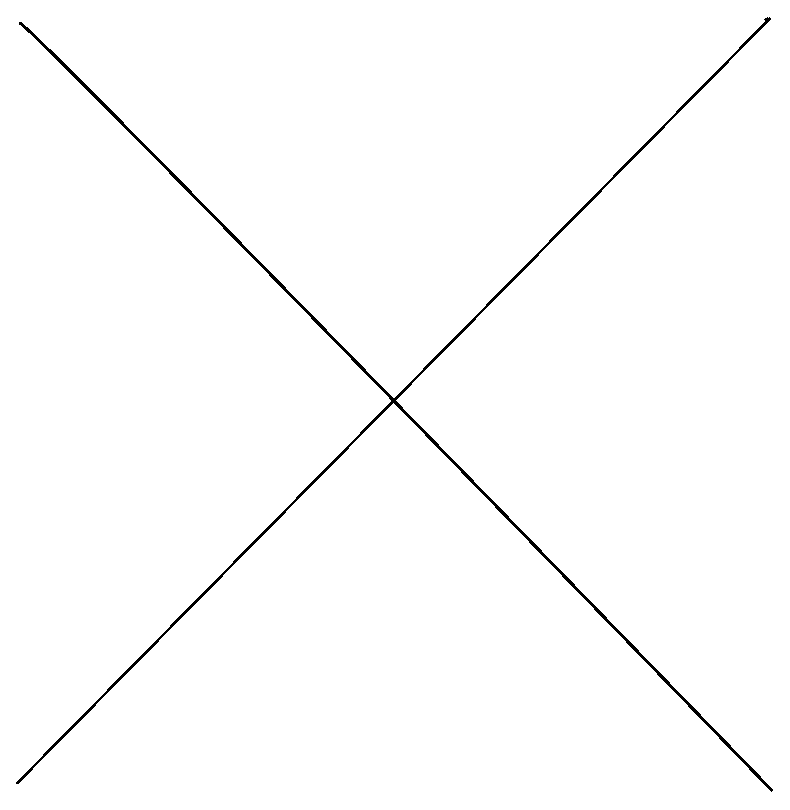
\includegraphics[width=\textwidth]{graphics/placeholder.eps}
\caption[An example of a champagne flow.]{An example of a champagne flow.}
\label{fig:champagne}
\end{figure}

\section{Shadowing}
\label{sec:shadowing}

Text to fix the formatting.

\begin{figure}
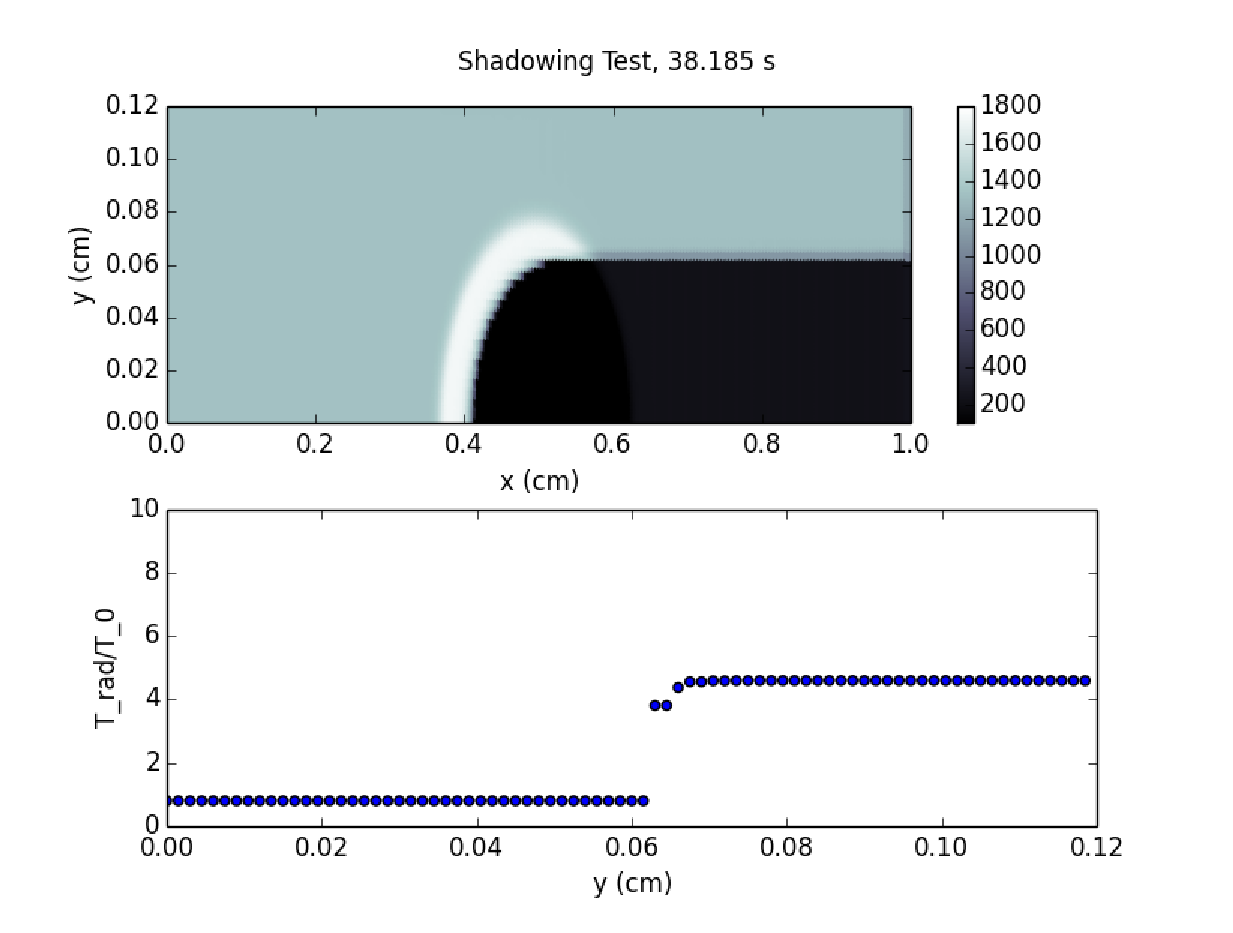
\includegraphics[width=\textwidth]{graphics/shadow10000.eps}
\caption[Shadowing.]{Demonstrating the codes ability to shadow.}
\label{fig:shadow}
\end{figure}

\section{Galaxy Disk}
\label{sec:galaxydisk}

Text to fix the formatting.

\section{Timings and Scaling}
\label{sec:timing}

Text to fix the formatting.

\begin{figure}
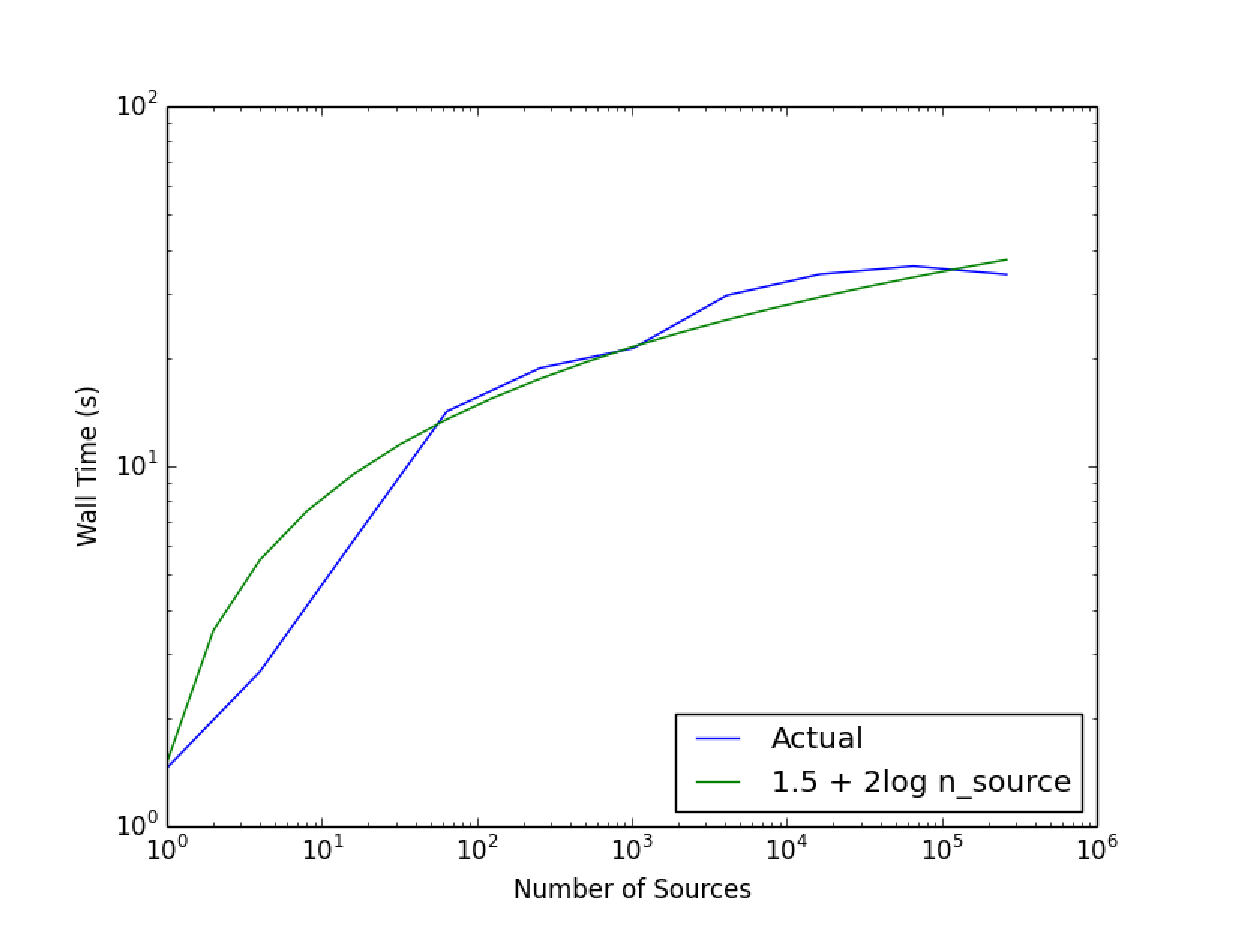
\includegraphics[width=\textwidth]{graphics/Timings.eps}
\caption[Wall time vs the number of sources.]{Wall time vs the number of sources.}
\label{fig:scaling}
\end{figure}

